%\documentclass{beamer}%[aspectratio=169]
\documentclass[aspectratio=169,mathserif]{beamer}  %[aspectratio=169]

% \usepackage{pgfpages} 
% \setbeameroption{show notes on second screen} 
%
% Choose how your presentation looks.
%
% For more themes, color themes and font themes, see:
% http://deic.uab.es/~iblanes/beamer_gallery/index_by_theme.html

%\mode<presentation>
%{
\usecolortheme{ruc} % or try albatross, beaver, crane, ...
%\usefonttheme{professionalfonts}  
\usefonttheme{serif} % default family is serif
\usepackage{fontspec}
%\setmainfont{Bitstream Vera Serif}
%\setmainfont{EB Garamond}
%\setmainfont{Baskerville}
\setmainfont{Georgia}
\setbeamertemplate{navigation symbols}{}
\setbeamertemplate{caption}[numbered]
\setbeamertemplate{footline}[frame number]
%} 
\usepackage[english]{babel}
\usepackage[utf8x]{inputenc}
\usepackage{subfigure}
\usepackage{color}
\usepackage{bm}
\usepackage{multirow}
\usepackage[absolute,overlay]{textpos}
  \setlength{\TPHorizModule}{1mm}
  \setlength{\TPVertModule}{1mm}

\usepackage{pgfpages}
% These slides also contain speaker notes. You can print just the slides,
% just the notes, or both, depending on the setting below. Comment out the want
% you want.
\setbeameroption{hide notes} % Only slides
%\setbeameroption{show only notes} % Only notes
%\setbeameroption{show notes on second screen=right} % Both  

\usepackage{amsmath}
\usepackage{amssymb}
\usepackage{amsfonts}
\usepackage{bm}
\usepackage{graphicx}
\usepackage{cancel}

\usepackage[backend=bibtex,sorting=none]{biblatex}
\addbibresource{references.bib}
\setbeamerfont{footnote}{size=\tiny}
\setbeamertemplate{bibliography item}[text]
\newcommand{\dd}{\mathrm{d}}
\newcommand{\R}{\mathbb{R}}
\newcommand{\E}{\mathbb{E}}
\newcommand{\light}[1]{\textcolor{gray}{#1}}
\newcommand{\tb}{\textbf}
\newcommand{\red}{\textcolor{red}}


\title[11.18Pre]{\huge{\textbf{Decoupled Contrastive Learning \\ $\&$ Debiased Contrastive Learning}}}
\author{
\tb{presenter}: Shen Yuan
}
\date{}


\begin{document} 


\begin{frame}
  \titlepage
  \vspace{-1cm}
  \centering
  \includegraphics[width=0.4\linewidth]{ruc_logo.png}\quad
  \includegraphics[width=0.4\linewidth]{GSAI_logo.png}
\end{frame}



\begin{frame}[noframenumbering]
\begin{itemize}
    \begin{LARGE}
    \item Understanding Contrastive Learning
    \item \light{Decoupled Contrastive Learning}
    \item \light{Debiased Contrastive Learning}
    \item \light{Summary}
    \end{LARGE}
\end{itemize}
\end{frame}



\begin{frame}{What is Contrastive Learning?}

\red{\tb{Contrastive learning}} is a machine learning technique used to learn the general features of a dataset \tb{without labels} by teaching the model which data points are similar or different.

\pause 

\begin{figure}[t]
\centerline{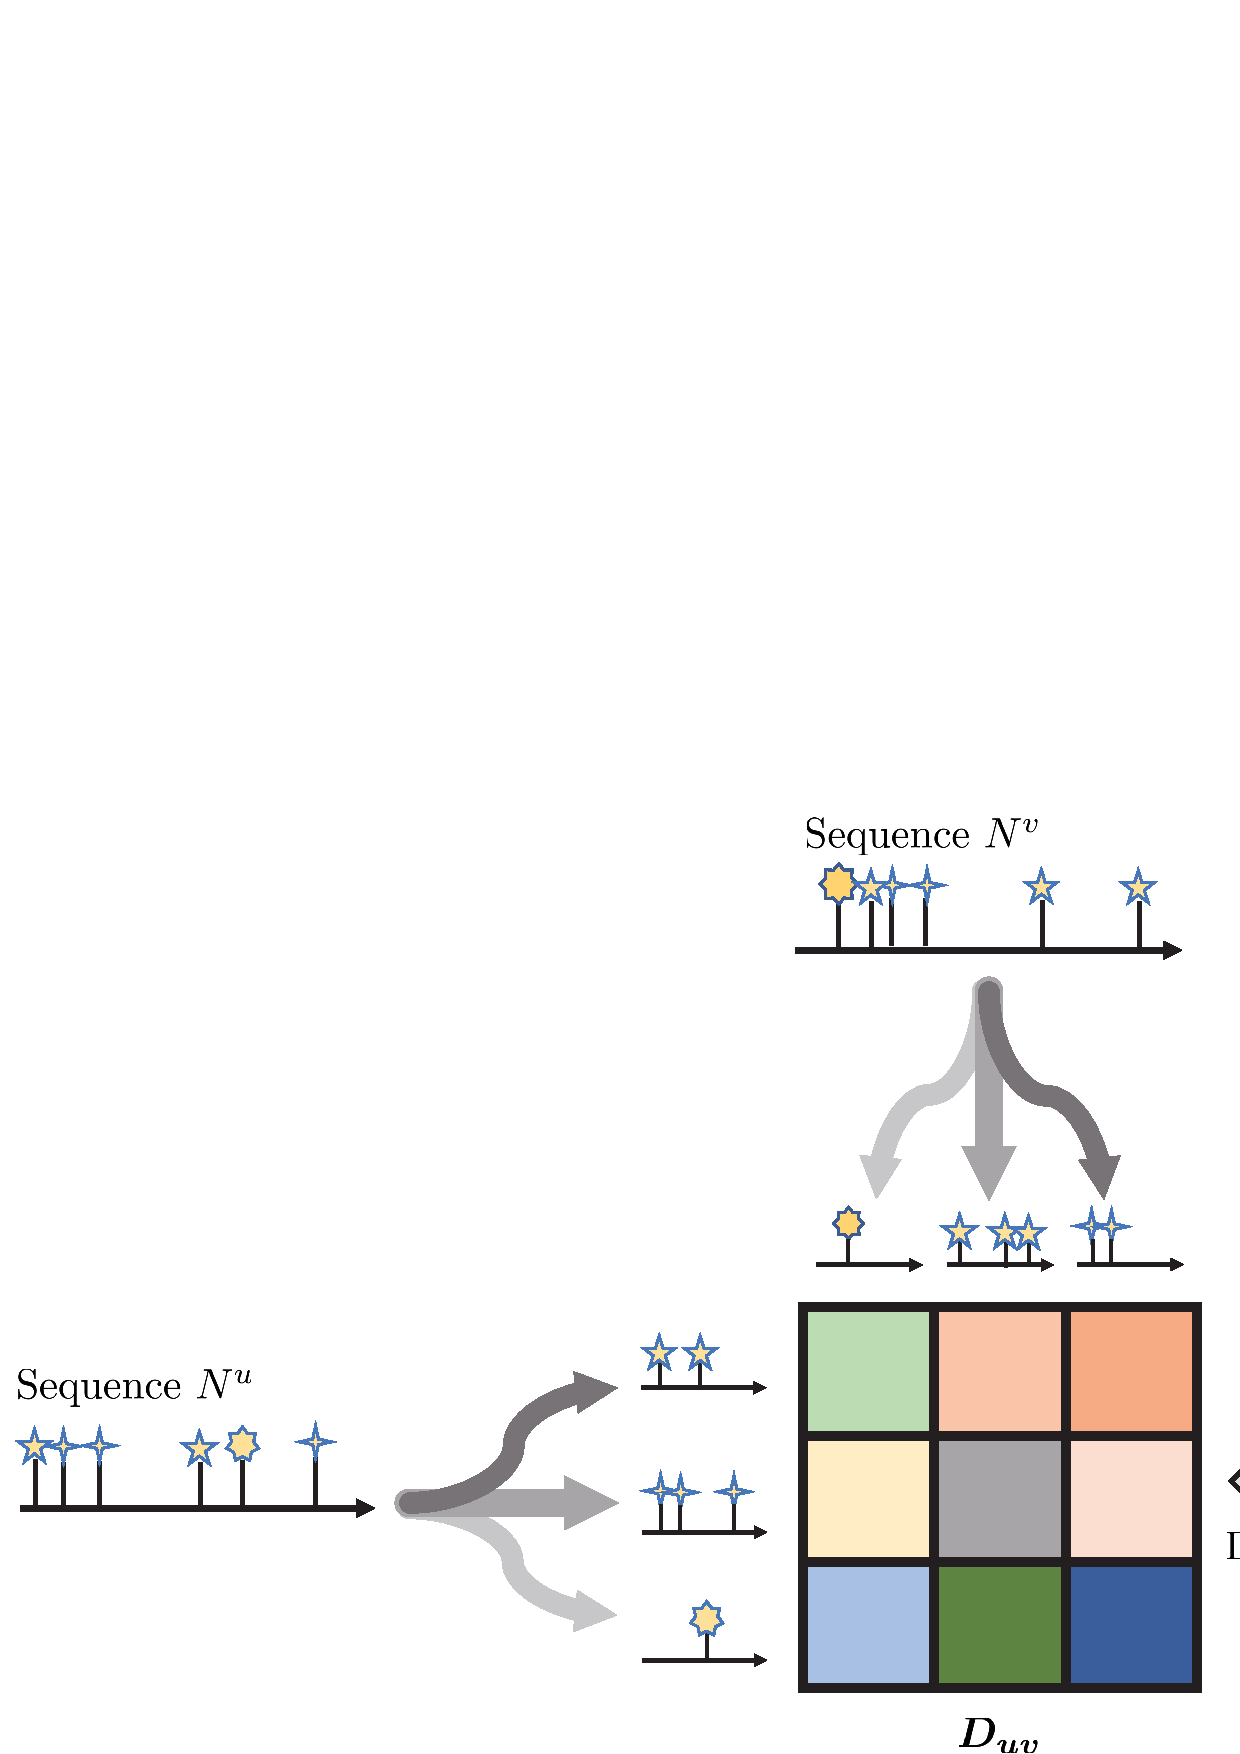
\includegraphics[width=0.7\linewidth]{figure2.png}}
\label{fig1}
\end{figure}

\end{frame}



\begin{frame}{What is Contrastive Learning?}

The aim of Contrastive Learning is to \tb{learn an encoder $\bm{f}(\cdot)$} such that:

\begin{figure}[t]
\centerline{\includegraphics[width=0.7\linewidth]{figure9.pdf}}
\label{fig1}
\end{figure}

\end{frame}



\begin{frame}{How does Contrastive Learning Work?}

In this part, we will focus on \tb{SimCLR}, one of the contrastive learning approaches proposed by the Google Brain Team. 

\pause

~\\
This framework consists of three basic steps:

\begin{itemize}
    \item data augmentaion
    \item encoding
    \item Loss minimization of representations
\end{itemize}

\end{frame}



\begin{frame}{SimCLR - Data Augmentation}

For each image in dataset, we can perform augmentation operations (i.e. crop, resize, recolor, etc.) to get \tb{two} augmented views. 

We want the model to learn that these two images are “similar” because they are actually different versions (or views) of the same image.

\begin{figure}[t]
\centerline{\includegraphics[width=0.7\linewidth]{figure4.png}}
\label{fig1}
\end{figure}

\end{frame}



\begin{frame}{SimCLR - Encoding}

Then, we can feed these two images into some deep learning models (i.e. encoder~$f(\cdot)$) to extract \tb{vector representations} for each image.

\begin{figure}[t]
\centerline{\includegraphics[width=0.7\linewidth]{figure3.png}}
\label{fig1}
\end{figure}

\end{frame}



\begin{frame}{SimCLR - Encoding}

\begin{columns}[T]
\begin{column}{0.4\textwidth}
\begin{itemize}[<+->]
    \item The framework SimCLR uses \tb{ResNet} as the encoder $f(\cdot)$ to encode two images as vector representations (i.e., $\bm{h=f(x)}$). 
    \item The output of the CNN is then inputted to a set of Dense Layers called the \tb{projection head}, $\bm{z=g(h)/\|g(h)\|_2}$ to transform the data into another space. This extra step is empirically shown to improve performance.
\end{itemize}
\end{column}
\begin{column}{0.55\textwidth}
    \includegraphics[width=\linewidth]{figure5.png}
\end{column}
\end{columns}

\end{frame}



\begin{frame}{SimCLR - Loss Minimization of Representations}

We can compute the probability that the two augmented images are similar by \tb{softmax} function.

\begin{center}
\includegraphics[width=0.7\linewidth]{figure11.pdf}   
\end{center}

\pause

\tb{Negative pairs} are created by combining our augmented images with \tb{all} of the other images in our batch.

\end{frame}



\begin{frame}{SimCLR - Loss Minimization of Representations}

Finally, the loss function of the two augmented images can be illustrated as follows

\begin{center}
\includegraphics[width=\linewidth]{figure8.png}   
\end{center}

\end{frame}




\begin{frame}{Similarity}

Generally, we compute the similarity between two vectors by \tb{cosine similarity},

\begin{eqnarray*}
\begin{aligned}
\text{similarity}(\bm{z_i, z_j})=\bm{\frac{\langle z_i, z_j \rangle}{\|z_i\|\|z_j\|}}
\end{aligned}    
\end{eqnarray*}

\end{frame}



\begin{frame}{SimCLR - More Mathematical Notations!}

Reformulate the loss function in a more mathematical form:

\pause

\begin{itemize}[<+->]
    \item given a batch of $N$ samples (e.g. images), $\{\bm{x}_1,\ldots,\bm{x}_N\}$
    \item let $\bm{x}_i^{(1)},\bm{x}_i^{(2)}$ be two augmented views of the sample $\bm{x}_i$ and $B$ be the set of all of the augmented views in the batch, i.e. $B=\{\bm{x}_i^{(k)}|k\in\{1,2\},i=1,\ldots,N\}$
    \item each of the views $\bm{x}_i^{(k)}$ is sent into the same encoder network $f$ and the output $\bm{h}_i^{(k)}=f(\bm{x}_i^{(k)})$ is then projected by a normalized MLP projector that $\bm{z}_i^{(k)}=g(\bm{h}_i^{(k)})/\|g(\bm{h}_i^{(k)})\|$
    \item For each augmented view $\bm{x}_i^{(k)}$, SimCLR solves a classification problem by using all the rest of views in $B$ as targets, and assigns the only positive label to $\bm{x}_i^{(u)}$, where $u\neq k$.
\end{itemize}


\end{frame}



\begin{frame}{SimCLR - More Mathematical Notations!}

SimCLR creates a cross-entropy loss function $L_i^{(k)}$ for each view $\bm{x}_i^{(k)}$, and the overall loss function is $L=\sum_{k\in \{1,2\}, i=1,\ldots,N} L_i^{(k)}$

\begin{eqnarray}
\begin{aligned}
L_i^{(k)}=-\log \frac{\exp (\langle \bm{z}_i^{(1)}, \bm{z}_i^{(2)} \rangle / \tau)}{\exp (\langle \bm{z}_i^{(1)}, \bm{z}_i^{(2)} \rangle / \tau) +\sum_{k\in \{1,2\},\ j=1,\ldots,N,\ j\neq i} \exp (\langle \bm{z}_i^{(k)}, \bm{z}_j^{(l)} \rangle / \tau)}
\end{aligned}
\end{eqnarray}


\end{frame}



\begin{frame}[noframenumbering]
\begin{itemize}
    \begin{LARGE}
    \item \light{Understanding Contrastive Learning}
    \item Decoupled Contrastive Learning
    \item \light{Debiased Contrastive Learning}
    \item \light{Summary}
    \end{LARGE}
\end{itemize}
\end{frame}



\begin{frame}{Decoupled Contrastive Learning - Motivation}

There exists a \tb{negative-positive coupling (NPC)} multiplier $q_{B,i}^{(1)}$ in the gradient of $L_i^{(1)}$:

\begin{eqnarray}
\begin{aligned}
\begin{cases}
-\nabla_{\bm{z}_i^{(1)}}L_i^{(1)}=\frac{\red{q_{B,i}^{(1)}}}{\tau}\left[\bm{z}_i^{(2)}-\sum_{l\in\{1,2\},\ j=1,\ldots,N,\ j\neq i} \frac{\exp (\langle \bm{z}_i^{(1)}, \bm{z}_j^{(l)} \rangle / \tau)}{\sum_{q\in \{1,2\},\ j=1,\ldots,N,\ j\neq i} \exp (\langle \bm{z}_i^{(1)}, \bm{z}_j^{(q)} \rangle / \tau)}\cdot\bm{z}_j^{(l)}\right]\\
-\nabla_{\bm{z}_i^{(2)}}L_i^{(1)}=\frac{\red{q_{B,i}^{(1)}}}{\tau} \cdot \bm{z}_i^{(1)}\\
-\nabla_{\bm{z}_j^{(l)}}L_i^{(1)}=-\frac{\red{q_{B,i}^{(1)}}}{\tau}\frac{\exp (\langle \bm{z}_i^{(1)}, \bm{z}_j^{(l)} \rangle / \tau)}{\sum_{q\in \{1,2\},\ j=1,\ldots,N,\ j\neq i} \exp (\langle \bm{z}_i^{(1)}, \bm{z}_j^{(q)} \rangle / \tau)}\cdot\bm{z}_i^{(1)}
\end{cases}
\end{aligned}
\end{eqnarray}

\pause

where the NPC multiplier $q_{B,i}^{(1)}$ is:

\begin{eqnarray}
\begin{aligned}
q_{B,i}^{(1)}=1-\frac{\exp (\langle \bm{z}_i^{(1)}, \bm{z}_i^{(2)} \rangle / \tau)}{\exp (\langle \bm{z}_i^{(1)}, \bm{z}_i^{(2)} \rangle / \tau) +\sum_{q\in \{1,2\},\ j=1,\ldots,N,\ j\neq i} \exp (\langle \bm{z}_i^{(1)}, \bm{z}_j^{(q)} \rangle / \tau)}
\end{aligned}
\end{eqnarray}

\end{frame}



\begin{frame}{Negative-positive Coupling (NPC) reduces efficiency}

\begin{center}
    \includegraphics[width=\linewidth]{figure12.png}
\end{center}

\pause

\begin{eqnarray*}
\begin{aligned}
q_{B,i}^{(1)}=1-\frac{\exp (\langle \bm{z}_i^{(1)}, \bm{z}_i^{(2)} \rangle / \tau)}{\exp (\langle \bm{z}_i^{(1)}, \bm{z}_i^{(2)} \rangle / \tau) +\sum_{q\in \{1,2\},\ j=1,\ldots,N,\ j\neq i} \exp (\langle \bm{z}_i^{(k)}, \bm{z}_j^{(q)} \rangle / \tau)}
\end{aligned}
\end{eqnarray*}

\end{frame}




\begin{frame}{Decoupled contrastive learning loss}

If we remove the NPC multiplier $q_{B,i}^{(k)}$, we reach a decoupled contrastive learning loss $L_{DC}=\sum_{k\in\{1,2\},\ i=1,\ldots,N}L_{DC,i}^{(k)}$, where $L_{DC,i}^{(k)}$ is :

\begin{eqnarray}
\begin{aligned}
L_{DC,i}^{(k)}
&=-\log \frac{\exp (\langle \bm{z}_i^{(1)}, \bm{z}_i^{(2)} \rangle / \tau)}{\cancel{\exp (\langle \bm{z}_i^{(1)}, \bm{z}_i^{(2)} \rangle / \tau)} +\sum_{k\in \{1,2\},\ j=1,\ldots,N,\ j\neq i} \exp (\langle \bm{z}_i^{(k)}, \bm{z}_j^{(l)} \rangle / \tau)}\\
&=-\langle \bm{z}_i^{(1)},\bm{z}_i^{(2)}\rangle/\tau + \log\sum_{k\in \{1,2\},\ j=1,\ldots,N,\ j\neq i} \exp (\langle \bm{z}_i^{(k)}, \bm{z}_j^{(l)} \rangle / \tau)
\end{aligned}
\end{eqnarray}

\end{frame}



\begin{frame}{Experiments}

\begin{center}
    \includegraphics[width=0.95\linewidth]{figure13.png}
\end{center}

\end{frame}



\begin{frame}{Experiments}

\begin{center}
    \includegraphics[width=0.9\linewidth]{figure14.png}
\end{center}

\end{frame}



\begin{frame}[noframenumbering]
\begin{itemize}
    \begin{LARGE}
    \item \light{Understanding Contrastive Learning}
    \item \light{Decoupled Contrastive Learning}
    \item Debiased Contrastive Learning
    \item \light{Summary}
    \end{LARGE}
\end{itemize}
\end{frame}



\begin{frame}{Debiased Contrastive Learning - Motivation}

When we create negative pairs $(x,x^-)$ after sampling positive pair $(x,x^+)$, we actually made an assumption that \tb{all the rest of images} are considered as negative samples \tb{NOT} ``similar'' with the given view $x$.

\pause

~\\
However, it's possible that $x^-$ is actually similar to $x$. 
    
\end{frame} 



\begin{frame}{Debiased Contrastive Learning - Motivation}

\begin{center}
    \includegraphics[width=0.9\linewidth]{figure15.png}
\end{center}
    
\end{frame}



\begin{frame}{Preliminary}

\begin{itemize}[<+->]
    \item Assume an \tb{underlying} set of discrete latent classes $\mathcal{C}$ that represent semantic content, i.e. similar pairs $(x,x^+)$ have the same latent class.
    \item Denoting the distribution over classes by $\rho(c)$, and the class probabilities $\rho(c)=\tau^+$ are \tb{uniform}(i.e. $\rho(c)=1/\|\mathcal{C}\|, c\in\mathcal{C}$), and let $\tau^-=1-\tau^+$ be the probability of observing any different class.
    \item $p_x^+(x')=\tau^+$ is the probability of observing $x'$ as a positive example for $x$ and $p_x^-(x')=\tau^-$ is the probability of a negative example.
\end{itemize}

\end{frame}



\begin{frame}{Unbiased Contrastive Loss}

For contrastive learning, the ideal loss to optimize would be

\begin{eqnarray}
\begin{aligned}
L_{\text{Unbiased}}^N(f)=\E_{\substack{x\sim p,\ x^+\sim p_x^+,\\ \red{x_i^-\sim p_x^-} }}\left[-\log \frac{e^{f(x)^\top f(x^+)}}{e^{f(x)^\top f(x^+)}+ \sum_{i=1}^{N}e^{f(x)^\top f(x_i^-)}} \right]
\end{aligned}
\end{eqnarray}


\pause

~\\
However, $x_i^-\sim p_x^-$ is not accessible.

\begin{eqnarray}
\begin{aligned}
L_{\text{biased}}^N(f)=\E_{\substack{x\sim p,\ x^+\sim p_x^+,\\ \red{x_i^-\sim p} }}\left[-\log \frac{e^{f(x)^\top f(x^+)}}{e^{f(x)^\top f(x^+)}+ \sum_{i=1}^{N}e^{f(x)^\top f(x_i^-)}} \right]
\end{aligned}
\end{eqnarray}
    
\end{frame}



\begin{frame}{Debiased Contrastive Loss}

Next, we derive a loss that is closer to the ideal $L_{\text{Unbiased}}^N$.

\pause
~\\
We can decompose the data distribution as

\begin{eqnarray}
\begin{aligned}
p(x')&=\tau^+p_x^+(x')+\tau^-p_x^-(x') \\ \pause
p_x^-(x')&=(p(x')-\tau^+p_x^+(x'))/\tau^-\\
p_x^-(x')&=\frac{1}{\tau^-}p(x')-\frac{\tau^+}{\tau^-}p_x^+(x')
\end{aligned}
\end{eqnarray}

\pause
~\\
Hence, $x_i^-\sim p_x^-$ can be replaced with that $x_i^-\sim p$ with probability $\frac{1}{\tau^-}$ and $x_i^-\sim p_x^+$ with probability $\frac{\tau^+}{\tau^-}$.

\end{frame}



\begin{frame}{Debiased Contrastive Loss}

Hence, $x_i^-\sim p_x^-$ can be replaced with that $x_i^-\sim p$ with probability $\frac{1}{\tau^-}$ and $x_i^-\sim p_x^+$ with probability $\frac{\tau^+}{\tau^-}$.

\begin{eqnarray}
\begin{aligned}
L_{\text{Unbiased}}^N(f)=\E_{\substack{x\sim p,\ x^+\sim p_x^+,\\ \red{x_i^-\sim p_x^-} }}\left[-\log \frac{e^{f(x)^\top f(x^+)}}{e^{f(x)^\top f(x^+)}+ \sum_{i=1}^{N}e^{f(x)^\top f(x_i^-)}} \right]
\end{aligned}
\end{eqnarray}

\pause

~\\
Leveraging Bernoulli distribution,
\begin{eqnarray}
\begin{aligned}
\frac{1}{(\tau^-)^N}\sum_{k=0}^N \left(\begin{matrix}N\\k\end{matrix}\right)(-\tau^+)^k\E_{\substack{x\sim p,\ x^+\sim p_x^+,\\ \red{\{x_i^-\}_{i=1}^k\sim p_x^+},\\ \red{\{x_i^-\}_{i=k+1}^N\sim p}}}\left[-\log \frac{e^{f(x)^\top f(x^+)}}{e^{f(x)^\top f(x^+)}+ \sum_{i=1}^{N}e^{f(x)^\top f(x_i^-)}} \right]
\end{aligned}
\end{eqnarray}

\end{frame}



\begin{frame}{Debiased Contrastive Loss}

We can use the empirical estimate $\tilde{L}_{\text{Debiased}}^N$ to approximate the real loss $L_{\text{Debiased}}^N$:

\begin{eqnarray}
\begin{aligned}
L_{\text{Debiased}}^N=&\E_{\substack{x\sim p,\ x^+\sim p_x^+,\\ \red{\{x_i^-\}_{i=1}^N\sim p_x^-}}}\left[-\log \frac{e^{f(x)^\top f(x^+)}}{e^{f(x)^\top f(x^+)}+ \red{\sum_{i=1}^{N}e^{f(x)^\top f(x_i^-)}}} \right]\\
\tilde{L}_{\text{Debiased}}^N= &\E_{\substack{x\sim p,\\ x^+\sim p_x^+}}\left[-\log \frac{e^{f(x)^\top f(x^+)}}{e^{f(x)^\top f(x^+)} + \red{N(\frac{1}{\tau^-}\E_{x^-\sim p}[e^{f(x)^\top  f(x^-)}]-\frac{\tau^+}{\tau^-}\E_{v\sim p_x^+}[e^{f(x)^\top f(v)}])}} \right]
\end{aligned}
\end{eqnarray}


\end{frame}



% \begin{frame}{Debiased Contrastive Learning - Motivation}



% \begin{eqnarray}
% \begin{aligned}
% L_{\text{Biased}}^N(f)\ge L_{\text{Unbiased}^N}(f) + \E_{x\sim p}\left[0\wedge\frac{\E_{x^+\sim p_x^+}\exp(f(x)^\top f(x^+))}{\E_{x^-\sim p_x^-}\exp(f(x)^\top f(x^-))}\right]-e^{3/2}\sqrt{\frac{\pi}{2N}}
% \end{aligned}
% \end{eqnarray}


    
% \end{frame}



\begin{frame}{Debiased Contrastive Loss}

With $N$ samples $\{u_i\}_{i=1}^N$ from $p$ and $M$ samples $\{v_i\}_{i=1}^M$ from $p_x^+$, we estimate the expectation of the second term in the denominator as

\begin{eqnarray}
\begin{aligned}
g(x,\{u_i\}_{i=1}^N,\{v_i\}_{i=1}^M)=\max\left\{\frac{1}{\tau^-}\left(\frac{1}{N}\sum_{i=1}^Ne^{f(x)^\top f(u_i)}-\tau^+\frac{1}{M}\sum_{i=1}^Me^{f(x)^\top f(v_i)},\ e^{-1/t}\right)\right\}
\end{aligned}
\end{eqnarray}

\pause

We constrain the estimator $g$ to be greater than its theoretical minimum $e^{-1/t}\leq e^{f(x)^\top f(x_i^-)}$ to prevent calculating the logarithm of a negative number.

\pause

\begin{eqnarray}
\begin{aligned}
L_{\text{Debiased}}^{N,M}(f)=\E_{\substack{x\sim p,\ x^+\sim p_x^+,\\ \red{\{u_i\}_{i=1}^N\sim p},\\ \red{\{v_i\}_{i=1}^M\sim p_x^+}}}\left[-\log \frac{e^{f(x)^\top f(x^+)}}{e^{f(x)^\top f(x^+)}+ \red{Ng(x,\{u_i\}_{i=1}^N,\{v_i\}_{i=1}^M)}} \right]
\end{aligned}
\end{eqnarray}

    
\end{frame}



\begin{frame}{Error bound}

\begin{eqnarray}
\begin{aligned}
\left|\tilde{L}_{\text{Debiased}}^N(f)-L_{\text{Debiased}}^{N,M}(f)\right|\leq\frac{e^{3/2}}{\tau^-}\sqrt{\frac{\pi}{2N}}+\frac{e^{3/2}\tau^+}{\tau^-}\sqrt{\frac{\pi}{2M}}
\end{aligned}
\end{eqnarray}

This inequality bounds the error due to finite $N$ and $M$ as decreasing with rate $\mathcal{O}(N^{-1/2}+M^{-1/2})$.
    
\end{frame}



\begin{frame}{Experiments - Image Classification}

\begin{center}
    \includegraphics[width=\linewidth]{figure16.png}
\end{center}
    
\end{frame}



% \begin{frame}{Experiments}

% \begin{center}
%     \includegraphics[width=\linewidth]{figure17.png}
% \end{center}
    
% \end{frame}



\begin{frame}{Experiments - Reinforcement Learning}

\begin{center}
    \includegraphics[width=\linewidth]{figure18.png}
\end{center}
    
\end{frame}



\begin{frame}{Summary}

Although the motivations of these two paper are different, they have similar solution. 

\begin{eqnarray}
\begin{aligned}
L^N(f)=\E_{\substack{x\sim p,\ x^+\sim p_x^+,\\ x_i^-\sim p }}\left[-\log \frac{e^{f(x)^\top f(x^+)}}{\red{e^{f(x)^\top f(x^+)}}+ \sum_{i=1}^{N}e^{f(x)^\top f(x_i^-)}} \right]
\end{aligned}
\end{eqnarray}
    
\end{frame}



\end{document}	% Done!

